\section{Methods}
\label{hptpcPaper:sec:Methods}
\begin{itemize}
    \item Discussion of experimental setup
\item Beamline
\item Beam Instrumentation
\item UsToF
\item DsToF
    \begin{itemize}
        \item Description of the DsToF scintillator and bar configuration 
        \item Brief outline of the DsToF DAQ system
        \item DsToF efficiencies with appropriate plot
    \end{itemize}

\item (Cursory) TPC description
\item MC overview
\item Analysis methods and supporting plots; examples of ToF plots, proton and pion peaks with MC

\end{itemize}

    The downstream time of flight (DsToF) system consists of 10 bars of plastic scintillator, which form the detector medium. Attached to either end of each of these scintillator bars is a 5" Hamamatsu R6594 photomultiplier tube. The bars are arranged in two rows of five, such that there is complete coverage for any beam particles incident upon the detector. Diagrams of the downstream time of flight system along with its dimensions are show in figure~\ref{fig:dstofFront} and~\ref{fig:dstofDiagonal}.
    
    The time resolution of the bars and PMTs was measured to be 1~ns. The spatial resolution of the bars and PMTs was measured to be 8.3~cm.
    
    \begin{figure}[ht]    
    	\begin{minipage}[t]{.48\textwidth}
    		\centering
    		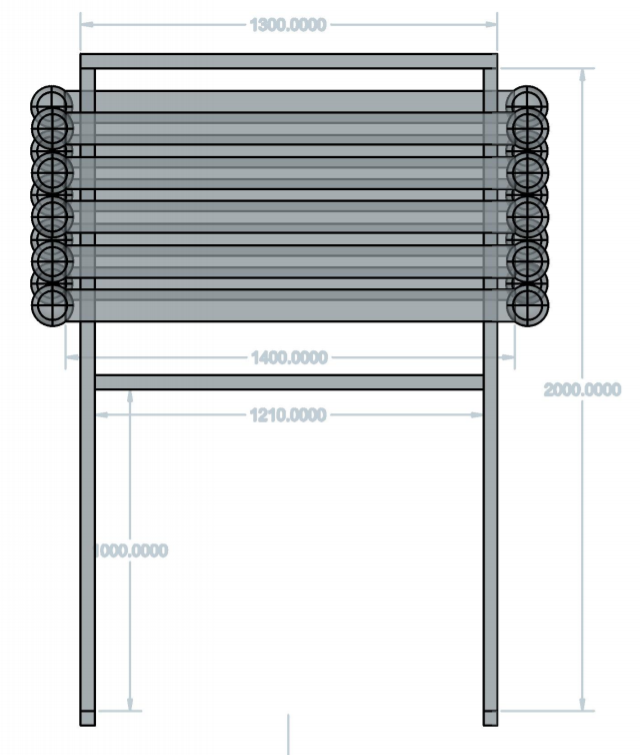
\includegraphics[width=0.6\linewidth]{files/Figures/dstofFront.png}
    		\caption{Front view of the downstream time of flight system}
    		\label{fig:dstofFront}
    	\end{minipage}
    	\hspace{0.3cm}
    	\begin{minipage}[t]{.48\textwidth}
    		\centering
    		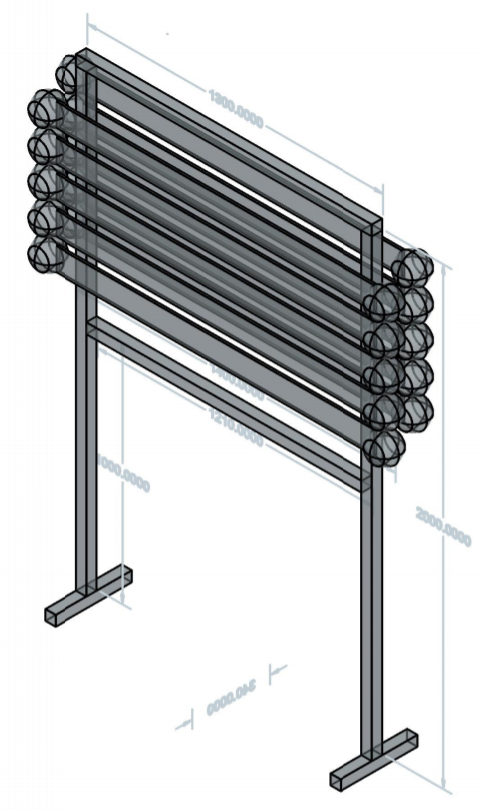
\includegraphics[width=0.45\linewidth]{files/Figures/dstofDiag.png}
    		\caption{Diagonal view of the downstream time of flight system showing more clearly the two rows of scintillator bars and photomultiplier tubes}
    		\label{fig:dstofDiagonal}
    	\end{minipage}
    \end{figure}
    
    All 20 of the photomultiplier tubes have their anode signals read out using NIM discriminators which are then fed into a time-to-digital converter. 
    
    A signal (i.e. an incident particle of any kind) in the downstream time of flight system was considered to have occurred if a signal was seen in both photomultiplier tubes on the same bar within 20~ns of each other.
    
    Additionally, a signal is also fed into the same time-to-digital converter whenever there is a coincidence between the $S_1$ and $S_2$ timing points. When calculating the time of flight of a given particle, this time of coincidence is used as first timing point.
    


